% Paper #1 - English manuscript draft.
% Build: tectonic main_en.tex   (XeTeX + BibTeX, see README.md)
\documentclass[a4paper,11pt]{article}

\usepackage{fontspec}
\setmainfont{texgyretermes}[Extension=.otf,UprightFont=*-regular,BoldFont=*-bold,ItalicFont=*-italic,BoldItalicFont=*-bolditalic]
\usepackage[english]{babel}
\setlength{\emergencystretch}{2em}
\usepackage{amsmath,amssymb}
\usepackage{graphicx}
\usepackage{booktabs}
\usepackage{multirow}
\usepackage[margin=2.4cm]{geometry}
\usepackage[numbers,sort&compress]{natbib}
\usepackage{caption}
\captionsetup{font=small,labelfont=bf}
\usepackage{tikz}
\usetikzlibrary{arrows.meta,positioning,fit}
\usepackage[colorlinks=true,linkcolor=blue!50!black,citecolor=blue!50!black,urlcolor=blue!50!black]{hyperref}

\newcommand{\nuot}{\nu_{12}}
\newcommand{\nuto}{\nu_{21}}
\newcommand{\RR}{R^2}

\title{Deep Generative Inverse Design of Auxetic Metamaterials: Navigating
Multi-Objective Demands and Out-of-Distribution Generalization}
\author{Trịnh Bình Minh\thanks{[Affiliation and corresponding-author details to be inserted.]}}
\date{Draft, \today}

\begin{document}
\maketitle

\begin{abstract}
Deep generative models can propose metamaterial unit cells for a target
effective property in milliseconds. A usable design, however, must
simultaneously match the target after binarization and finite-element (FE)
verification, be manufacturable, and ideally be obtainable for targets outside
the training data. We study these three demands for two-dimensional auxetic
unit cells generated by a conditional variational autoencoder (cVAE)
fine-tuned with differentiable homogenization. For accuracy, we show that
test-time latent refinement must optimize the verified design: refining the
continuous decoder output drives the objective to $\sim\!10^{-10}$ while the
verified error stays six orders of magnitude larger, whereas embedding the
verification operators in the objective raises the FE-verified $\RR$ of
$\nuot$ on 100 held-out targets from 0.874 to 0.998 (single sample) and from
0.986 to 0.997 (best of 30). For multi-objective selection, a weighted
accuracy--manufacturability--aesthetics score agrees moderately with an
independent Pareto ranking (median Spearman 0.71). For out-of-distribution
targets, the cVAE generates designs with the correct, unseen sign of the
Poisson ratio where nearest-neighbour retrieval cannot, but it does not
extrapolate magnitudes beyond the training range.
\end{abstract}

\noindent\textbf{Keywords:} Auxetic metamaterials; Deep generative models;
Differentiable physics; Inverse design; Topology optimization; Homogenization

% ---------------------------------------------------------------------------
\section{Introduction}

Auxetic metamaterials contract laterally under uniaxial compression. Their
negative Poisson's ratio originates in the microarchitecture rather than the
chemistry of the constituent material
\citep{lakes1987foam,evans2000auxetic,bertoldi2017flexible}. Inverse
homogenization by topology optimization is the classical route from a
prescribed effective tensor to a unit cell
\citep{sigmund1994materials,larsen1997design,bendsoe2003topology}, but every
new target requires an iterative optimization with hundreds of FE solves.
Data-driven inverse design amortizes this cost: variational autoencoders,
generative adversarial networks and diffusion models trained on simulated
libraries return candidate architectures almost instantly
\citep{wang2020deep,mao2020gan,kumar2020spinodoid,bastek2022inverting,kollmann2020deep,zheng2021controllable,pahlavani2024deep,bastek2023diffusion}.

Practical use places three demands on such a generator, and they are rarely
examined together.
\emph{(i) Verified accuracy.} What is manufactured is a binarized,
resampled version of the generated density field, so accuracy must be judged
by FE analysis of that design, not by a learned surrogate. Surrogates of the
forward map are known to be exploitable by optimizers and generators
\citep{trabucco2021coms}. Single samples also rarely meet tight tolerances,
so pipelines generate many candidates and select among them with FE
\citep{pahlavani2024deep}.
\emph{(ii) Multiple objectives.} A design that meets the target but contains
floating islands, sub-resolution struts or edges that do not tile is
unusable. Accuracy therefore has to be traded against manufacturability and,
at lower priority, against geometric regularity.
\emph{(iii) Out-of-distribution (OOD) targets.} The main argument for a
generative model over a lookup in the training library is that it might
produce designs for targets the library does not contain. Whether it does,
and along which directions of property space, is an empirical question.

This paper addresses the three demands with one pipeline and one evaluation
protocol, in which every reported number is FE-verified on the binarized
design and every comparison carries a paired confidence interval. Our
contributions are:
\begin{enumerate}
\item \textbf{Binarization-aware latent refinement.} We refine the latent
code of a frozen cVAE using exact analytic gradients of a periodic
homogenization solver. We show that refinement is only reliable when the
objective is evaluated on the verified design, obtained through periodic-edge
enforcement, Heaviside projection with continuation
\citep{guest2004achieving,wang2011projection} and nearest-neighbour
resampling. We also provide direct evidence of the grey-density exploitation
that occurs otherwise.
\item \textbf{Multi-objective selection with an external check.} We rank
candidates by a weighted score of accuracy, manufacturability and aesthetics.
We test this score against an independent Pareto ranking instead of assuming
that it is adequate.
\item \textbf{A physically grounded OOD characterization.} We show that
symmetric targets with $\nuot=\nuto\le-1$ are inadmissible for orthotropic
cells, which invalidates naive ``extreme'' benchmarks. We then separate
generalization in the \emph{sign} of the Poisson ratio, where the cVAE
succeeds and retrieval fails, from generalization in \emph{magnitude}, where
all methods saturate at the edge of the training data.
\item \textbf{Controlled negative results.} Neither a Kolmogorov--Arnold
network (KAN) head nor an implicit wavelet (WIRE) decoder improves on the
convolutional baseline under FE-verified metrics.
\end{enumerate}

% ---------------------------------------------------------------------------
\section{Results}

\subsection{Framework and evaluation protocol}

Figure~\ref{fig:framework} shows the pipeline. A cVAE maps a target pair
$(\nuot^{*},\nuto^{*})$ and a latent vector $z\sim\mathcal N(0,I)$ to a
$64\times64$ density image. The cVAE is trained in two stages, the second
with a loss computed by FE homogenization of prior samples (Methods). For
each target, $N$ latents are decoded and post-processed. Post-processing
consists of periodic-edge enforcement, thresholding at 0.5 and
nearest-neighbour resampling to the $50\times50$ FE grid. Each candidate is
then FE-homogenized and scored for manufacturability and aesthetics. The
best candidate by a composite score is optionally refined in latent space,
and a refined design is kept only if its verified error is lower (``guarded''
refinement).

All accuracy numbers are FE-verified on the binarized design. The
in-distribution benchmark (IN100) comprises 100 held-out test conditions
drawn with a fixed seed. Comparisons report paired bootstrap 95\% confidence
intervals (CI) over conditions \citep{efron1993bootstrap}. Success criteria
were fixed before each experiment (Methods).

\begin{figure}[t]
\centering
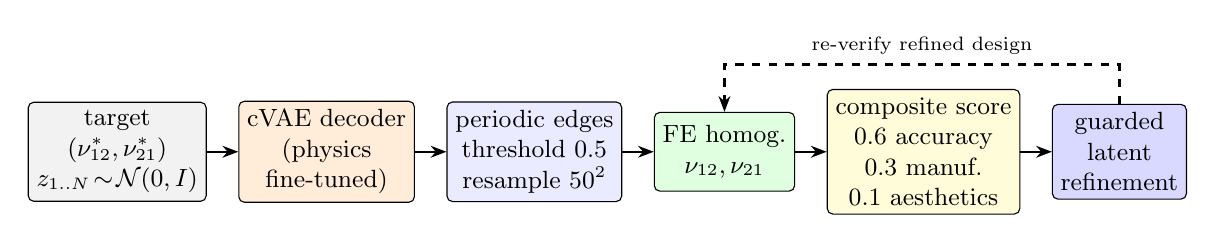
\begin{tikzpicture}[
  node distance=3mm and 4mm,
  box/.style={draw, rounded corners=2pt, align=center, font=\small,
              minimum height=10mm, inner sep=3pt, fill=#1},
  box/.default=white,
  arr/.style={-{Stealth[length=2mm]}, thick}]
\node[box=gray!10] (t) {target\\$(\nu_{12}^{*},\nu_{21}^{*})$\\$z_{1..N}\!\sim\!\mathcal N(0,I)$};
\node[box=orange!15, right=of t] (g) {cVAE decoder\\(physics\\fine-tuned)};
\node[box=blue!8, right=of g] (v) {periodic edges\\threshold 0.5\\resample $50^2$};
\node[box=green!12, right=of v] (fe) {FE homog.\\$\nu_{12},\nu_{21}$};
\node[box=yellow!15, right=of fe] (s) {composite score\\0.6 accuracy\\0.3 manuf.\\0.1 aesthetics};
\node[box=blue!15, right=of s] (r) {guarded\\latent\\refinement};
\draw[arr] (t) -- (g);
\draw[arr] (g) -- (v);
\draw[arr] (v) -- (fe);
\draw[arr] (fe) -- (s);
\draw[arr] (s) -- (r);
\draw[arr, dashed] (r.north) -- ++(0,5mm) -| node[pos=0.25, above, font=\scriptsize]{re-verify refined design} (fe.north);
\end{tikzpicture}
\caption{Inverse-design pipeline. Every candidate is verified by FE
homogenization after the same post-processing that a manufactured design
would undergo. Selection combines verified accuracy with manufacturability
(connectivity, minimum feature size, periodicity) and a low-weight aesthetic
score. Refinement is detailed in Fig.~\ref{fig:pipeline}.}
\label{fig:framework}
\end{figure}

\subsection{Verified accuracy requires optimizing the verified design}

\paragraph{Continuous refinement exploits grey densities.}
Refining the continuous decoder output (30 L-BFGS steps
\citep{liu1989lbfgs}, gradients through the decoder and the exact
homogenization sensitivities) helps single samples of the production model.
On IN100, $\RR(\nuot)$ rises from 0.874 to 0.976 and the mean absolute error
(MAE) of $\nuot$ falls by 57.7\% (95\% CI 49.4--64.6\%;
Table~\ref{tab:main}, Fig.~\ref{fig:parity}b). The same refinement, however,
\emph{worsens} the best-of-30 winner. MAE($\nuot$) rises from 0.0152 to
0.0246, a change of $-62.5\%$ (CI $-98.3$ to $-33.9\%$), and $\RR$ drops from
0.986 to 0.968. The objective trace explains why
(Fig.~\ref{fig:gap}). At the end of continuous refinement the median
objective is $2.5\times10^{-10}$, but the median verified squared error of
the binarized design is $4.4\times10^{-4}$. The optimizer matches the target
on a field whose intermediate densities do not survive thresholding. This is
the same failure mode as surrogate exploitation, arising inside an exact
physics model.

\paragraph{Binarization-aware refinement.}
Placing differentiable counterparts of the verification operators inside the
objective (Fig.~\ref{fig:pipeline}; 32 steps over $\beta\in\{1,4,16,64\}$)
reduces the objective--verification gap by three orders of magnitude
(Fig.~\ref{fig:gap}). All pre-registered in-distribution criteria are met
(Table~\ref{tab:main}).
\begin{itemize}
\item \textbf{Single samples.} $\RR(\nuot)$ rises from 0.874 to 0.998 and
MAE($\nuot$) falls by 91.8\% (CI 89.0--93.9\%). The mean relative error of
$\nuot$ drops from 14.4\% to 2.6\%, and $\RR(\nuto)$ rises from 0.477 to
0.883.
\item \textbf{After best-of-30.} MAE($\nuot$) falls by 62.6\% (CI
50.7--72.1\%) and $\RR(\nuot)$ rises from 0.986 to 0.997. Guarded refinement
accepts 92\% of refinements and reduces MAE($\nuot$) by 69.1\% (CI
61.6--75.4\%), without extra FE solves.
\end{itemize}
After best-of-30, MAE($\nuto$) decreases from 0.0327 to 0.0128, whereas
$\RR(\nuto)$ falls from 0.802 to 0.712. A few conditions therefore acquire
larger $\nuto$ deviations, which the guarded rule, based on the summed error,
does not always reject. Refinement costs 77 FE solves per condition on
average. With 50--100\,ms per solve including sensitivities on the
$50\times50$ grid, this amounts to a few seconds per design.

\begin{figure}[t]
\centering
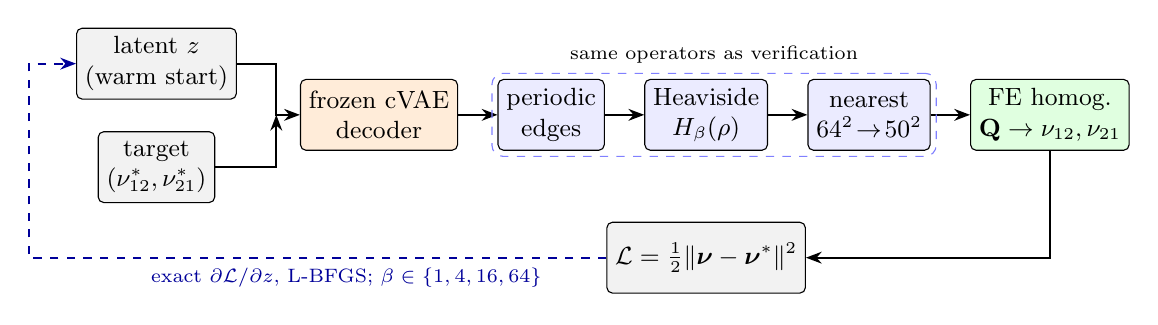
\begin{tikzpicture}[
  node distance=4mm and 5mm,
  box/.style={draw, rounded corners=2pt, align=center, font=\small,
              minimum height=9mm, inner sep=3pt, fill=#1},
  box/.default=white,
  arr/.style={-{Stealth[length=2mm]}, thick},
  grad/.style={-{Stealth[length=2mm]}, thick, dashed, blue!60!black}]
\node[box=gray!10] (z) {latent $z$\\(warm start)};
\node[box=gray!10, below=of z] (c) {target\\$(\nu_{12}^{*},\nu_{21}^{*})$};
\node[box=orange!15, right=8mm of z, yshift=-6.5mm] (dec) {frozen cVAE\\decoder};
\node[box=blue!8, right=of dec] (per) {periodic\\edges};
\node[box=blue!8, right=of per] (hv) {Heaviside\\$H_\beta(\rho)$};
\node[box=blue!8, right=of hv] (rs) {nearest\\$64^2\!\to\!50^2$};
\node[box=green!12, right=of rs] (fe) {FE homog.\\$\mathbf{Q}\to\nu_{12},\nu_{21}$};
\node[box=gray!10, below=9mm of hv] (loss) {$\mathcal{L}=\tfrac12\lVert\boldsymbol{\nu}-\boldsymbol{\nu}^{*}\rVert^2$};
\draw[arr] (z) -| ([xshift=-3mm]dec.west) -- (dec.west);
\draw[arr] (c) -| ([xshift=-3mm]dec.west);
\draw[arr] (dec) -- (per);
\draw[arr] (per) -- (hv);
\draw[arr] (hv) -- (rs);
\draw[arr] (rs) -- (fe);
\draw[arr] (fe.south) |- (loss.east);
\draw[grad] (loss.west) -- ([xshift=-6mm]loss.west -| z.west)
  node[pos=0.45, below, font=\scriptsize]{exact $\partial\mathcal{L}/\partial z$, L-BFGS; $\beta\in\{1,4,16,64\}$}
  |- (z.west);
\node[draw=blue!50, dashed, rounded corners, fit=(per)(hv)(rs), inner sep=2pt,
      label={[font=\scriptsize]above:same operators as verification}] {};
\end{tikzpicture}
\caption{Binarization-aware latent refinement. The frozen decoder output
passes through differentiable counterparts of the verification operators
before FE homogenization, so the quantity optimized is the quantity verified.
The continuous variant omits the dashed block and uses bilinear resampling.
Verification replaces $H_\beta$ by a hard threshold at 0.5.}
\label{fig:pipeline}
\end{figure}

\begin{table}[t]
\centering
\caption{FE-verified accuracy on IN100 (100 held-out targets, production
cVAE). $\Delta$MAE is the relative reduction of MAE($\nuot$) versus the
unrefined design of the same mode, with a paired bootstrap 95\% CI (10\,000
resamples). Negative values mean that refinement made results worse. FE
calls are per condition and include selection.}
\label{tab:main}
\small
\setlength{\tabcolsep}{4pt}
\begin{tabular}{llccccr}
\toprule
Mode & Refinement & $\RR(\nuot)$ & MAE($\nuot$) & $\RR(\nuto)$ & $\Delta$MAE [95\% CI] & FE calls\\
\midrule
\multirow{3}{*}{Single sample}
 & none                 & 0.874 & 0.0517 & 0.477 & -- & 1\\
 & continuous           & 0.976 & 0.0219 & 0.643 & $+57.7\%$ [49.4, 64.6] & 51\\
 & binarization-aware   & \textbf{0.998} & \textbf{0.0043} & \textbf{0.883} & $\mathbf{+91.8\%}$ [89.0, 93.9] & 78\\
\midrule
\multirow{4}{*}{Best-of-30}
 & none                 & 0.986 & 0.0152 & 0.802 & -- & 30\\
 & continuous           & 0.968 & 0.0246 & 0.637 & $-62.5\%$ [$-98.3$, $-33.9$] & 79\\
 & binarization-aware   & 0.997 & 0.0057 & 0.712 & $+62.6\%$ [50.7, 72.1] & 107\\
 & \quad guarded        & \textbf{0.998} & \textbf{0.0047} & -- & $\mathbf{+69.1\%}$ [61.6, 75.4] & 107\\
\bottomrule
\end{tabular}
\end{table}

\begin{figure}[t]
\centering
\includegraphics[width=\linewidth]{figures/fig_parity_en.pdf}
\caption{FE-verified versus target $\nuot$ on IN100 ($n=100$, single samples
of the production cVAE): (a) unrefined; (b) after continuous refinement;
(c) after binarization-aware refinement. All panels start from the same
latent code per condition. Dashed line: identity.}
\label{fig:parity}
\end{figure}

\begin{figure}[t]
\centering
\includegraphics[width=0.55\linewidth]{figures/fig_gap_en.pdf}
\caption{Objective--verification gap. Each point is one IN100 condition. The
horizontal axis shows the final refinement objective; the vertical axis
shows the squared Poisson-ratio error of the binarized design measured by an
independent FE solve. Continuous refinement (circles) reaches objectives
near $10^{-10}$ while verified errors remain at $10^{-4}$--$10^{-2}$.
Binarization-aware refinement (squares) moves points towards the identity.
Values below $10^{-14}$ are clipped for display.}
\label{fig:gap}
\end{figure}

\subsection{Multi-objective demands: manufacturability and composite ranking}

Accurate designs are not automatically buildable. Each candidate is checked
for (a) connectivity without struts thinner than two pixels and (b)
periodicity, meaning that opposite edges must match so that the cell tiles
by translation (Methods). On an earlier cVAE without periodic enforcement,
only 0--3.5\% of generated samples passed both checks. This rate was uniform
across property space, so the problem lies in decoder behaviour rather than
in data coverage. Enforcing periodicity by averaging opposite edges before
binarization is a training-free operation that raised the pass rate by more
than an order of magnitude. It is part of every verification in this paper.
With it, 24.7\% of the samples of the production model pass all checks
(300 test targets, $N=30$; Table~\ref{tab:multi}). In-distribution,
periodic enforcement therefore does not force a trade-off against accuracy.

Among the candidates for a target, selection maximizes the composite score
$0.6\,s_{\mathrm{acc}}+0.3\,s_{\mathrm{man}}+0.1\,s_{\mathrm{aes}}$. The
weights encode the priority order accuracy $>$ manufacturability $>$
aesthetics; they are a design choice, not a learned quantity. To test
whether this scalarization respects the multi-objective structure, we
computed, for 24 targets with 30 candidates each, the Spearman correlation
between the composite score and the non-dominated sorting rank over the
three raw objectives (Fig.~\ref{fig:spearman}). All 24 correlations were
positive (range 0.43--0.89). The median was 0.714, but the mean of 0.693
fell just short of the pre-registered threshold of 0.7. The composite score
therefore agrees moderately, not strongly, with the Pareto structure. That
the selected candidate always lies on the first Pareto front is guaranteed
mathematically for positive weights, so it is not evidence.

\begin{table}[t]
\centering
\caption{Multi-objective indicators. Upper block: production pipeline with
periodic enforcement and best-of-30 selection on 300 test targets.
Manufacturable fraction: share of generated samples passing connectivity,
minimum-feature and periodicity checks. Hit rate: fraction of targets whose
first sample is auxetic ($\nuot<0$). Lower block: agreement of the composite
score with Pareto ranks (24 targets $\times$ 30 candidates).}
\label{tab:multi}
\small
\begin{tabular}{lccc}
\toprule
Model & $\RR(\nuot)$, best-of-30 & Single-sample hit rate & Manufacturable fraction\\
\midrule
Production cVAE (dataset v2)    & 0.995 & 0.997 & 0.247\\
Earlier cVAE (dataset v1)       & 0.998 & 0.983 & 0.280\\
\midrule
\multicolumn{4}{p{0.85\linewidth}}{Composite score vs.\ Pareto rank: Spearman mean 0.693, median 0.714, range 0.43--0.89; 24/24 targets positive.}\\
\bottomrule
\end{tabular}
\end{table}

\begin{figure}[t]
\centering
\includegraphics[width=0.5\linewidth]{figures/fig_spearman_en.pdf}
\caption{Distribution over 24 targets of the Spearman correlation between the
composite score and the Pareto rank of 30 candidates (objectives: verified
$|\Delta\nuot|$, manufacturability score, aesthetic score). Dotted:
pre-registered threshold for the mean.}
\label{fig:spearman}
\end{figure}

\subsection{Out-of-distribution generalization}

\paragraph{Admissible targets.}
Before testing extrapolation we asked which targets exist. For a
two-dimensional orthotropic material, positive definiteness of the
compliance requires $\nuot\nuto<1$ \citep{lempriere1968poisson}. Symmetric
targets $\nuot^{*}=\nuto^{*}\le-1$ are therefore infeasible. In the training
data the most negative $\nuot=-1.95$ is paired with $\nuto=-0.04$, and the
largest product $\nuot\nuto$ is 0.43. This matters for benchmarking. An
earlier ``extreme auxetic'' test in our project used targets such as
$(-2.1,-2.1)$ and $(-2.2,-1.6)$, all six of which violate the bound. Its
failures therefore say nothing about extrapolation, and we exclude them
here. Out-of-range magnitude targets below are anisotropic, with
$\nuto^{*}=-0.05$.

\paragraph{Sign: the cVAE generalizes, retrieval cannot.}
Every training sample is auxetic ($-1.95\le\nuot\le-0.002$). For six
non-auxetic targets with $0.1\le\nuot^{*}\le0.8$, nearest-neighbour retrieval
from the 57\,216-sample training library necessarily returns the sample
closest to zero ($\nuot=-0.002$), with the wrong sign for every target. The
cVAE (best of 10) produced positive $\nuot$ for all six targets
(Table~\ref{tab:signflip}, Fig.~\ref{fig:signflip}), with MAE 0.19 versus 0.40
for retrieval. The attained magnitude, however, saturates near 0.3. For
$\nuot^{*}=0.8$ the cVAE reached 0.30. The cVAE thus extrapolates the
\emph{direction} of the property but not its full magnitude. This test used
an earlier checkpoint (dataset v1) and six targets, and should be read as
qualitative evidence.

\begin{table}[t]
\centering
\caption{Sign-flip OOD targets (training data contain only $\nuot<0$).
FE-verified $\nuot$ of nearest-neighbour retrieval and of the cVAE (first
sample and best of 10); last column: manufacturable fraction of the 10 cVAE
samples.}
\label{tab:signflip}
\small
\begin{tabular}{cccccc}
\toprule
$(\nuot^{*},\nuto^{*})$ & Retrieval & cVAE, first & cVAE, best of 10 & Manuf.\\
\midrule
(0.1, 0.1) & $-0.002$ & 0.082 & 0.104 & 0.6\\
(0.3, 0.3) & $-0.002$ & 0.183 & 0.204 & 0.6\\
(0.5, 0.5) & $-0.002$ & 0.191 & 0.280 & 0.8\\
(0.8, 0.8) & $-0.002$ & 0.241 & 0.301 & 0.6\\
(0.2, 0.5) & $-0.002$ & 0.225 & 0.194 & 0.9\\
(0.5, 0.2) & $-0.002$ & 0.109 & 0.177 & 0.6\\
\midrule
MAE($\nuot$) & 0.402 & 0.237 & \textbf{0.191} & \\
\bottomrule
\end{tabular}
\end{table}

\begin{figure}[t]
\centering
\includegraphics[width=0.5\linewidth]{figures/fig_signflip_en.pdf}
\caption{Sign-flip generalization for symmetric non-auxetic targets. Retrieval
is bounded by the training library ($\nuot\le-0.002$). The cVAE reaches the
correct sign but saturates in magnitude. Dashed: identity.}
\label{fig:signflip}
\end{figure}

\paragraph{Magnitude: all methods saturate at the training boundary.}
We swept $\nuot^{*}\in\{-1.0,$ $-1.5,$ $-1.75,$ $-2.0,$ $-2.25,$ $-2.5\}$ ($\nuto^{*}=-0.05$)
with ten independent latent draws per target, best-of-30 selection and
periodic enforcement (Table~\ref{tab:ood}, Fig.~\ref{fig:ood}). Inside the
training range, binarization-aware refinement lowers the median relative
error of $\nuot$ to 0.2--0.4\%. Beyond the training minimum of $-1.95$, every
variant saturates. The most negative verified $\nuot$ among all 30 designs
at $\nuot^{*}=-2.5$ was $-1.99$. Unguarded refinement is then worse than no
refinement (32.4\% versus 22.5\% at $-2.5$). The guarded variant meets the
pre-registered 8\% criterion at $-2.0$ (4.9\%), but only because this target
lies 0.05 beyond the boundary; from $-2.25$ onwards it merely matches
best-of-30. Refinement is a local search in the decoder's latent space and
cannot create magnitudes the decoder never learned to represent.

\begin{table}[t]
\centering
\caption{Anisotropic magnitude sweep ($\nuto^{*}=-0.05$; best-of-30 with
periodic enforcement; 10 repeats per target). Entries: median relative error
of FE-verified $\nuot$. The training range of $\nuot$ ends at $-1.95$.}
\label{tab:ood}
\small
\begin{tabular}{lcccccc}
\toprule
$\nuot^{*}$ & $-1.0$ & $-1.5$ & $-1.75$ & $-2.0$ & $-2.25$ & $-2.5$\\
\midrule
Best-of-30, no refinement        & 0.5\% & 0.9\% & 4.1\% & 11.0\% & 16.1\% & 22.5\%\\
+ continuous refinement          & 1.4\% & 1.3\% & 3.2\% & 36.5\% & 38.9\% & 43.9\%\\
+ binarization-aware refinement  & 0.4\% & 0.2\% & 0.3\% & 12.5\% & 22.3\% & 32.4\%\\
+ binarization-aware, guarded    & 0.2\% & 0.2\% & 0.3\% & \textbf{4.9\%} & 14.8\% & 21.9\%\\
\bottomrule
\end{tabular}
\end{table}

\begin{figure}[t]
\centering
\includegraphics[width=0.62\linewidth]{figures/fig_ood_en.pdf}
\caption{Median relative error of FE-verified $\nuot$ versus target
($\nuto^{*}=-0.05$). Error bars: interquartile range over 10 latent draws per
target; markers offset horizontally for legibility. Shaded: outside the
training range. Dotted: pre-registered 8\% criterion at $\nuot^{*}=-2.0$.}
\label{fig:ood}
\end{figure}

\subsection{Architecture ablations}

\paragraph{KAN versus linear heads.}
We replaced the three linear layers of the cVAE (latent mean, log-variance
and decoder bottleneck) with Kolmogorov--Arnold layers \citep{liu2024kan}.
Both heads were trained with identical recipes, hyperparameters and seeds
(123 and 7). KAN was declared the winner only if the paired CI excluded zero
for both seeds. It did not win in any mode (Table~\ref{tab:kan}). In the
production mode (best-of-30 without refinement), the linear head was
significantly better for both seeds. With refinement, both heads reached
$\RR(\nuot)=0.997$--$0.999$. The KAN head has $3.2\times$ more parameters
(4.79\,M versus 1.49\,M) and needs about $1.6\times$ the time per epoch, so
we retain the linear head.

\begin{table}[t]
\centering
\caption{Controlled KAN versus linear ablation on IN100 (two seeds).
$\Delta$MAE: relative reduction of MAE($\nuot$) of KAN versus linear
(positive favours KAN), paired bootstrap 95\% CI. Bold: CI excludes zero.}
\label{tab:kan}
\small
\setlength{\tabcolsep}{4pt}
\begin{tabular}{lcccc}
\toprule
 & \multicolumn{2}{c}{$\RR(\nuot)$ Linear / KAN} & \multicolumn{2}{c}{$\Delta$MAE KAN vs.\ Linear}\\
\cmidrule(lr){2-3}\cmidrule(lr){4-5}
Mode & seed 123 & seed 7 & seed 123 & seed 7\\
\midrule
Single sample              & 0.852 / 0.904 & 0.815 / 0.911 & $+13.3\%$ [$-0.2$, 24.4] & $\mathbf{+18.2\%}$ [3.8, 30.4]\\
Single sample + refinement & 0.994 / 0.997 & 0.998 / 0.999 & $+33.2\%$ [$-15.1$, 60.5] & $\mathbf{+33.9\%}$ [11.7, 52.3]\\
Best-of-30                 & 0.977 / 0.974 & 0.982 / 0.980 & $\mathbf{-25.2\%}$ [$-56.2$, $-1.0$] & $\mathbf{-19.9\%}$ [$-42.1$, $-1.7$]\\
Best-of-30 + refinement    & 0.998 / 0.997 & 0.998 / 0.999 & $+11.3\%$ [$-38.7$, 43.6] & $\mathbf{+44.1\%}$ [24.9, 59.7]\\
\bottomrule
\end{tabular}
\end{table}

\paragraph{Implicit wavelet decoder.}
A resolution-agnostic WIRE decoder \citep{saragadam2023wire} was given one
final attempt. It combined Heaviside projection inside the physics loss, no
forced symmetry and the two-stage recipe. The pre-registered criteria were a
single-sample hit rate of at least 30\% and a positive FE $\RR$ on 24
held-out targets. It reached a hit rate of 12.5\% and an FE $\RR$ of $-7.19$
after best-of-30, against about 99.7\% hit rate for the convolutional
decoder. Only 4.6\% of its samples were manufacturable. We therefore closed
this direction.

% ---------------------------------------------------------------------------
\section{Discussion}

\paragraph{Accuracy.}
The central methodological finding is that physics-based refinement of a
generated design must evaluate its objective on the same object that will be
verified. Differentiating an exact solver removes surrogate error but not the
mismatch between a continuous decoder output and a binarized unit cell.
Fig.~\ref{fig:gap} shows that this mismatch lets the optimizer reach
objectives of $10^{-10}$ on a field that the verifier sees very differently.
The problem is invisible in the loss curve and only surfaces when a strong
baseline is refined. The ingredients of the remedy are standard in
density-based topology optimization
\citep{guest2004achieving,wang2011projection}. What is new is applying them
to the output of a frozen generative model during latent search, together
with the exact resampling and periodic post-processing used at verification.
The same principle should extend to any post-processing step that is
included in the verification.

\paragraph{Multiple objectives.}
The pipeline handles the three objectives at different stages.
Periodicity is enforced by construction, connectivity and feature size enter
through the composite score, and accuracy is improved last by refinement
that keeps the periodic edges. This ordering is pragmatic, and our evidence
for it is partial. The composite score agrees only moderately with the
Pareto ranking. The rank-based normalization of the accuracy term within
each candidate pool is a plausible cause that we have not yet tested. We
also have not measured whether refinement changes connectivity or feature
size. Designers who need guaranteed manufacturability can still restrict
selection to candidates that pass all checks. In earlier experiments this
required large candidate pools ($N\approx1500$) and lowered accuracy.

\paragraph{Out-of-distribution generalization.}
Our results suggest a more precise version of the common claim that
generative models ``generalize''. Along the sign of the Poisson ratio, the
cVAE produces designs in a region with zero training density, which a lookup
method cannot do by construction. Along magnitude, the generator, its
refinement and best-of-$N$ selection all stop at the training boundary. OOD
claims should therefore state the direction in property space and should
first check that the target is physically admissible. Magnitude
extrapolation will likely require new training data near the boundary, for
example from topology optimization seeded by generated designs, rather than
better sampling from the current model.

\paragraph{Limitations.}
(i) All analyses use linear-elastic, small-strain homogenization of
two-dimensional cells on a $50\times50$ grid with a base-material Poisson
ratio of 0.3. Large strain and three-dimensional architectures are not
addressed.
(ii) Designs are verified numerically, including against an independent FE
implementation, but not experimentally.
(iii) The sign-flip test used six targets and an earlier checkpoint. The
magnitude sweep used ten repeats per target.
(iv) The aesthetic score is a simple heuristic (mirror symmetry and boundary
smoothness) and has not been validated against human judgement.
(v) In-distribution, nearest-neighbour retrieval is highly competitive in
accuracy, so the advantage of a generative model shown here is specific to
out-of-distribution sign changes.
(vi) Refinement adds about 77 FE solves per target. This is inexpensive in
2D but would require efficient adjoint solvers in 3D.

% ---------------------------------------------------------------------------
\section{Methods}

\subsection{Data generation}
Unit cells were generated by SIMP topology optimization
\citep{bendsoe1989optimal,sigmund2001code,andreassen2011efficient} with a
density filter \citep{bourdin2001filters}, periodic boundary conditions and
energy-based homogenization
\citep{guedes1990preprocessing,andreassen2014homogenization,xia2015design}.
Auxetic objectives were minimized from four seed topologies, using the
optimality-criteria update or the method of moving asymptotes
\citep{svanberg1987mma} depending on the seed. Process parameters (volume
fraction, penalization, filter radius, move limit, void size, lattice
rotation) were screened by Latin hypercube sampling \citep{mckay1979lhs} and
refined in an adaptive multi-batch design of experiments using Sobol'
sequences \citep{sobol1967distribution} and optimized Latin hypercubes.
Samples with oscillatory convergence, degenerate topologies or labels outside
the physical range were removed. The $50\times50$ density fields were
box-filtered to $64\times64$ images and labelled with the homogenized
$(\nuot,\nuto)$. The production dataset contains 13\,624 unique cells, split
70/15/15 by seed family (2\,044 test samples). Training images are augmented
sixfold by rotations and reflections, with $\nuot\leftrightarrow\nuto$
swapped under $90^{\circ}$ rotations, giving 57\,216 training samples.

\subsection{Homogenization and exact sensitivities}
Density fields $\rho\in[0,1]^{50\times50}$ are discretized with bilinear
quadrilateral elements and the modified SIMP interpolation
$E(\rho)=E_{\min}+\rho^{p}(E_0-E_{\min})$ with $E_{\min}=10^{-9}E_0$, $p=3$
and $\nu_0=0.3$. The homogenized stiffness $\mathbf{Q}$ follows from three
periodic load cases through element mutual energies \citep{xia2015design}.
Poisson ratios are obtained from $\mathbf{S}=\mathbf{Q}^{-1}$ as
$\nuot=-S_{12}/S_{11}$ and $\nuto=-S_{12}/S_{22}$, which remains valid for
rotated, fully anisotropic cells. Because the energy formulation is
self-adjoint, the sensitivities $\partial\mathbf{Q}/\partial\rho_e$ are
available without extra solves. They are propagated analytically through
$\partial\mathbf{S}=-\mathbf{S}\,(\partial\mathbf{Q})\,\mathbf{S}$ and the
quotient rule in a custom PyTorch \citep{paszke2019pytorch} autograd
function, whose gradients agree with finite differences to a relative error
below $10^{-4}$. The solver agrees with an independent scikit-fem
\citep{gustafsson2020skfem} implementation to $10^{-9}$ on 24 designs.

\subsection{Conditional VAE}
The cVAE \citep{kingma2014vae,sohn2015cvae} is conditioned on
$c=(\nuot,\nuto)$ and has a 32-dimensional latent space. The encoder
consists of four convolution--batch-norm--ReLU--pooling blocks (32 to 256
channels) that keep a $4\times4$ spatial map, followed by linear layers for
the mean and log-variance. The decoder mirrors the encoder with transposed
convolutions and a sigmoid output. Stage 1 trains with binary cross-entropy
reconstruction, a KL term with linear warm-up \citep{bowman2016generating}
and a property-consistency term from a frozen convolutional surrogate
(weight $\gamma=20$; surrogate test $\RR$ of 0.974 for $\nuot$ and 0.964 for
$\nuto$). Stage 2 resumes from stage 1 and adds the squared error between
$c$ and the FE-homogenized Poisson ratios of decoded \emph{prior} samples
$z\sim\mathcal N(0,I)$ (weight 20; 8 samples every second epoch). This is
the regime used at inference, and training with this loss from scratch
fails. Optimization uses Adam \citep{kingma2015adam}. Checkpoints are
selected by FE-verified $\RR$ on validation conditions rather than by
validation loss, which the KL warm-up makes unreliable.

\subsection{Verification, manufacturability and composite score}
A decoded image is verified by (1) periodic-edge enforcement, in which
opposite boundary columns and then rows are replaced by their mean; (2)
thresholding at 0.5; (3) nearest-neighbour resampling to $50\times50$ with the
index map of the imaging library used to build the dataset; and (4) FE
homogenization. Manufacturability combines three checks on the binary image:
a single connected solid phase, a minimum feature size of two pixels
(morphological erosion), and periodicity (at most 10\% mismatched pixels
between opposite edges). The graded score $s_{\mathrm{man}}$ is the mean of
the three indicators. The aesthetic score $s_{\mathrm{aes}}$ averages mirror
symmetry about both axes and an inverse normalized perimeter-to-area ratio
computed with periodic wrap-around. The accuracy score $s_{\mathrm{acc}}$ is
$|\Delta\nuot|$ min--max normalized within the candidate pool, with sign
reversed so that higher is better. The Pareto validation applies iterated
non-dominated sorting to the three raw objectives and correlates the
resulting rank with the composite score per target.

\subsection{Latent refinement}
Given $\boldsymbol\nu^{*}$ and a starting latent $z_0$ (single sample or
best-of-$N$ winner), we minimize
\begin{equation}
\mathcal L_\beta(z)=\tfrac12\bigl\lVert
\boldsymbol\nu\bigl(\mathcal R\circ H_\beta\circ\mathcal P\circ D(z,c)\bigr)
-\boldsymbol\nu^{*}\bigr\rVert_2^2 ,
\end{equation}
where $D$ is the frozen decoder, $\mathcal P$ the (linear) periodic-edge
enforcement, $\mathcal R$ the nearest-neighbour resampling implemented as a
differentiable gather with an identical index map, and
\begin{equation}
H_\beta(\rho)=\frac{\tanh(\beta\eta)+\tanh\bigl(\beta(\rho-\eta)\bigr)}
{\tanh(\beta\eta)+\tanh\bigl(\beta(1-\eta)\bigr)},\qquad \eta=0.5,
\end{equation}
the smoothed Heaviside projection \citep{wang2011projection}. Thirty-two
L-BFGS steps (step size 0.5, strong-Wolfe line search) are split evenly
across $\beta\in\{1,4,16,64\}$, and L-BFGS is restarted at each level
because curvature information from a softer projection does not carry over.
The continuous baseline applies the loss to $D(z,c)$ with bilinear
resampling for 30 steps. Guarded refinement keeps the refined design only if
its verified $|\Delta\nuot|+|\Delta\nuto|$ is smaller than that of the start.

\subsection{Out-of-distribution protocols and retrieval baseline}
Retrieval returns the training sample with the smallest Euclidean distance
to the target in $(\nuot,\nuto)$. The sign-flip test used six non-auxetic
targets, 10 cVAE samples per target and FE-oracle selection. The magnitude
sweep used six anisotropic targets with $\nuto^{*}=-0.05$ and ten
independent repeats of best-of-30 per target. Admissibility was checked
against $\nuot\nuto<1$ \citep{lempriere1968poisson}.

\subsection{Statistics and pre-registration}
IN100 consists of 100 test conditions drawn with seed 123. Relative MAE
reductions and 95\% CIs are computed by paired percentile bootstrap over
conditions with 10\,000 resamples \citep{efron1993bootstrap}. An
improvement is claimed only if the CI excludes zero. Criteria were recorded
before each experiment. They were: at least 20\% MAE reduction for single
samples; no significant MAE increase after best-of-30; a median relative
error of at most 8\% at $\nuot^{*}=-2.0$; a mean Spearman correlation of at
least 0.7 for the composite score; for KAN, a CI excluding zero for both
seeds; and for WIRE, a hit rate of at least 30\% with FE $\RR>0$. L-BFGS on
GPU is not bit-wise deterministic, and repeated runs differed by about 0.006
in $\RR$.

\section*{Data and code availability}
Code, trained checkpoints and all per-condition outputs underlying the
tables and figures will be made available at [repository URL to be
inserted].

\section*{Acknowledgements and competing interests}
[To be completed.]

\bibliographystyle{unsrtnat}
\bibliography{refs}

\end{document}
